\documentclass{standalone}
\usepackage{tikz}
\usetikzlibrary{patterns, positioning}
\usepackage[sfdefault]{ClearSans} %% option 'sfdefault' activates Clear Sans as the default text font
\usepackage[T1]{fontenc}

\begin{document}
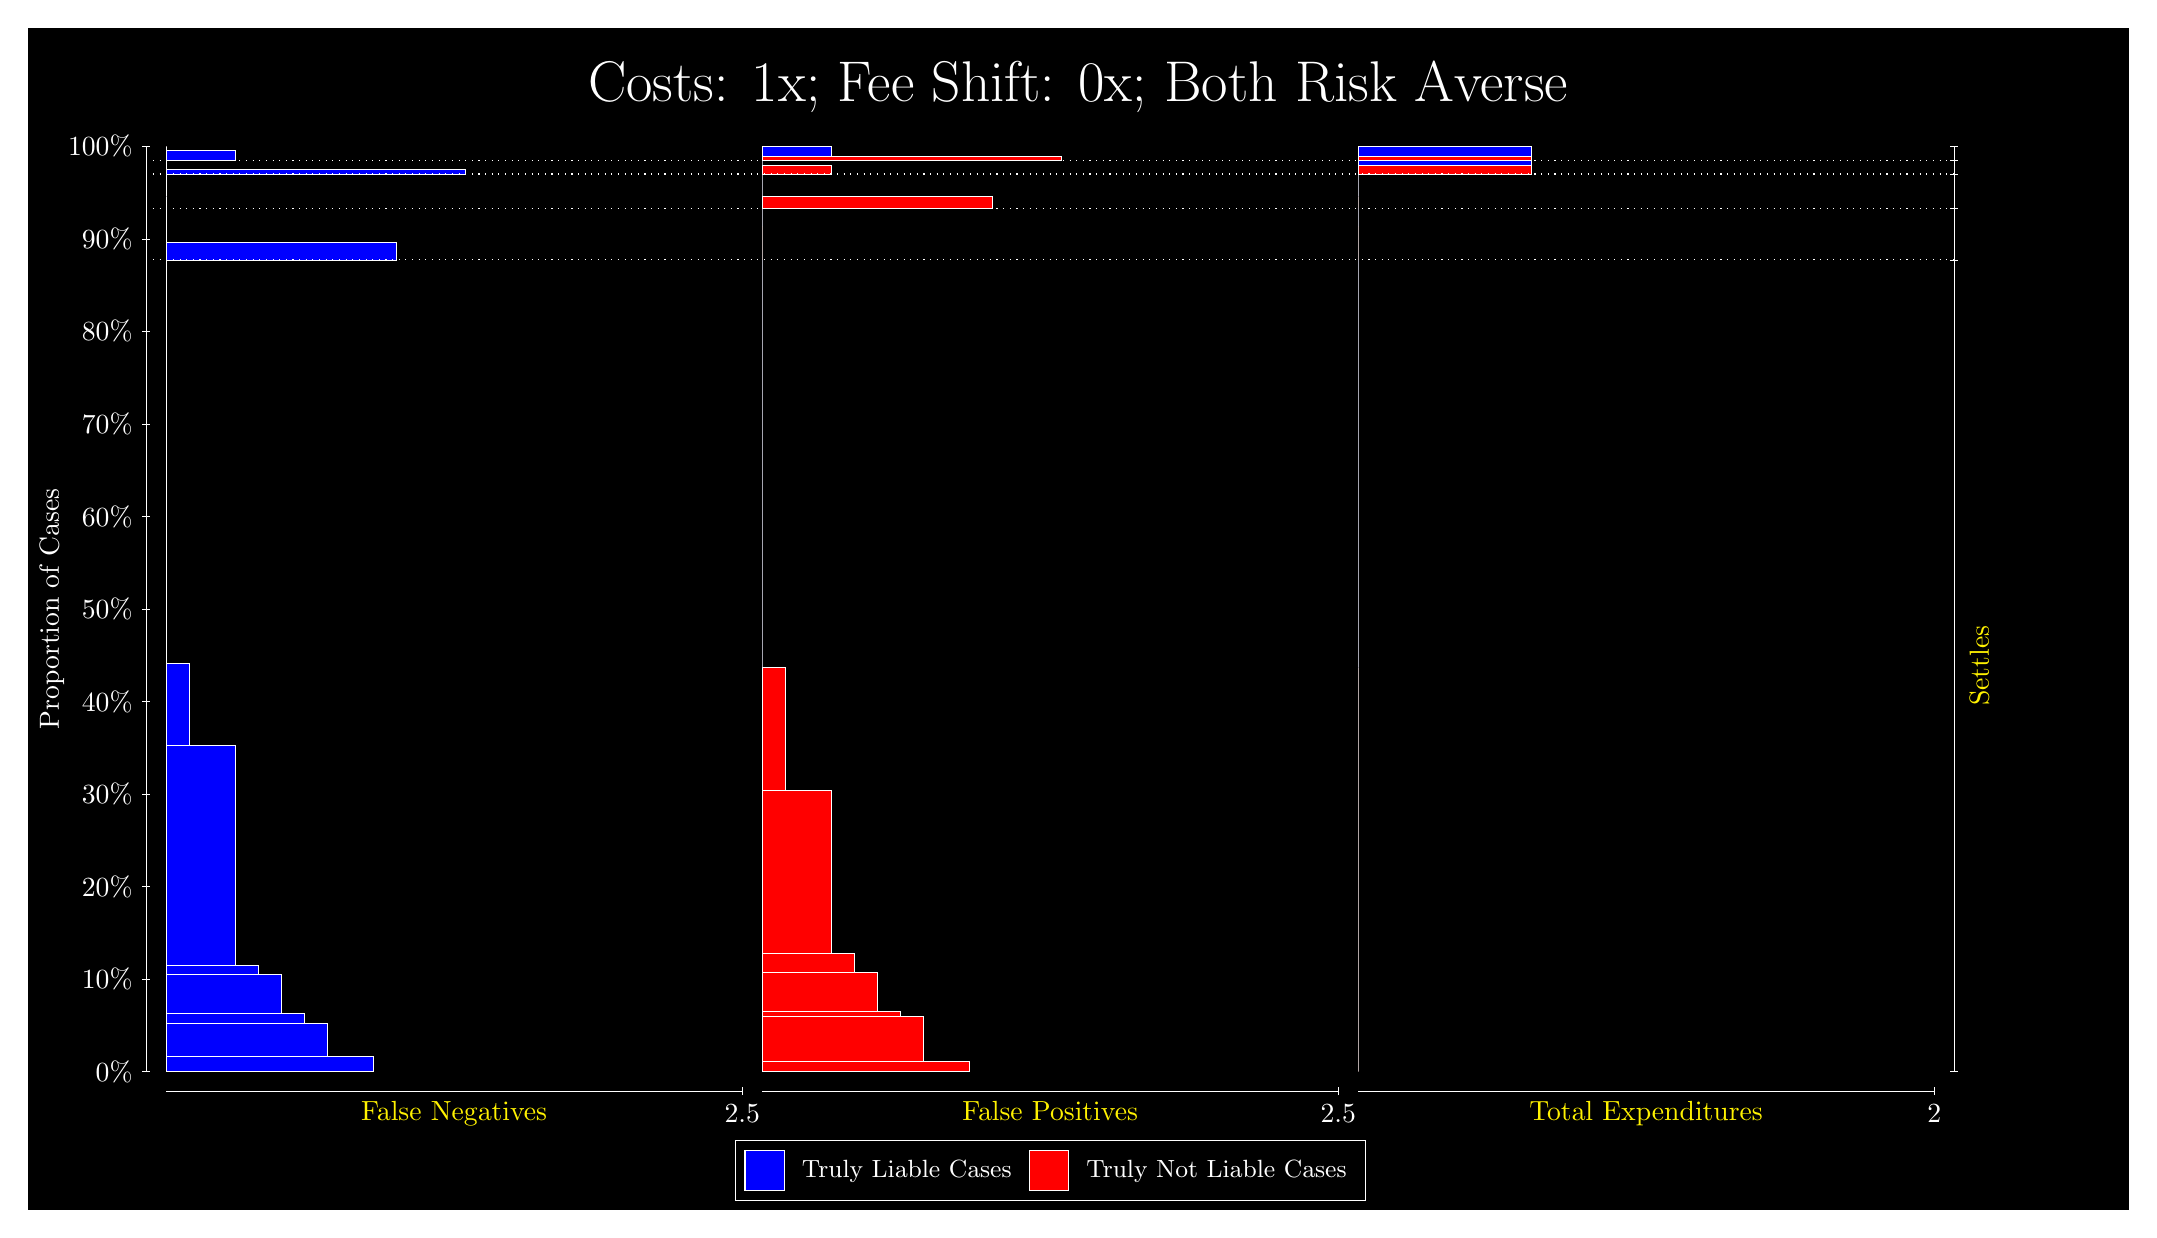
\begin{tikzpicture}
\draw[fill=black] (0,0) rectangle (26.667,15);
\draw[text=white] (0,13.5) rectangle (26.667,15) node[midway] {\huge Costs: 1x; Fee Shift: 0x; Both Risk Averse};
\draw[white, very thin] (1.5,1.75) -- (1.5,13.5);
\node[rotate=90, text=white, anchor=center] at (0.3, 7.625) {Proportion of Cases};
\draw[white, very thin] (1.45,1.75) -- (1.55,1.75);
\node[text=white, anchor=east] at (1.45, 1.75) {0\%};
\draw[white, very thin] (1.45,2.925) -- (1.55,2.925);
\node[text=white, anchor=east] at (1.45, 2.925) {10\%};
\draw[white, very thin] (1.45,4.1) -- (1.55,4.1);
\node[text=white, anchor=east] at (1.45, 4.1) {20\%};
\draw[white, very thin] (1.45,5.275) -- (1.55,5.275);
\node[text=white, anchor=east] at (1.45, 5.275) {30\%};
\draw[white, very thin] (1.45,6.45) -- (1.55,6.45);
\node[text=white, anchor=east] at (1.45, 6.45) {40\%};
\draw[white, very thin] (1.45,7.625) -- (1.55,7.625);
\node[text=white, anchor=east] at (1.45, 7.625) {50\%};
\draw[white, very thin] (1.45,8.8) -- (1.55,8.8);
\node[text=white, anchor=east] at (1.45, 8.8) {60\%};
\draw[white, very thin] (1.45,9.975) -- (1.55,9.975);
\node[text=white, anchor=east] at (1.45, 9.975) {70\%};
\draw[white, very thin] (1.45,11.15) -- (1.55,11.15);
\node[text=white, anchor=east] at (1.45, 11.15) {80\%};
\draw[white, very thin] (1.45,12.325) -- (1.55,12.325);
\node[text=white, anchor=east] at (1.45, 12.325) {90\%};
\draw[white, very thin] (1.45,13.5) -- (1.55,13.5);
\node[text=white, anchor=east] at (1.45, 13.5) {100\%};

\draw[white, very thin] (24.457,1.75) -- (24.457,13.5);
\draw[white, very thin] (24.407,1.75) -- (24.507,1.75);
\node[anchor=west] at (24.407, 1.75) {};
\draw[white, very thin] (24.407,12.058) -- (24.507,12.058);
\node[anchor=west] at (24.407, 12.058) {};
\draw[white, very thin] (24.407,12.714) -- (24.507,12.714);
\node[anchor=west] at (24.407, 12.714) {};
\draw[white, very thin] (24.407,13.149) -- (24.507,13.149);
\node[anchor=west] at (24.407, 13.149) {};
\draw[white, very thin] (24.407,13.317) -- (24.507,13.317);
\node[anchor=west] at (24.407, 13.317) {};
\draw[white, very thin] (24.407,13.5) -- (24.507,13.5);
\node[anchor=west] at (24.407, 13.5) {};

\draw[white, very thin, fill=blue] (1.75,1.75) rectangle (4.3848,1.9488);
\draw[white, very thin, fill=blue] (1.75,1.9488) rectangle (3.7993,2.3604);
\draw[white, very thin, fill=blue] (1.75,2.3604) rectangle (3.5065,2.49);
\draw[white, very thin, fill=blue] (1.75,2.49) rectangle (3.2138,2.9856);
\draw[white, very thin, fill=blue] (1.75,2.9856) rectangle (2.921,3.1023);
\draw[white, very thin, fill=blue] (1.75,3.1023) rectangle (2.6283,5.8995);
\draw[white, very thin, fill=blue] (1.75,5.8995) rectangle (2.0428,6.9301);
\draw[white, very thin, fill=red] (1.75,6.9301) rectangle (1.75,12.058);
\draw[white, very thin, fill=blue] (1.75,12.058) rectangle (4.6775,12.284);
\draw[white, very thin, fill=red] (1.75,12.284) rectangle (1.75,12.714);
\draw[white, very thin, fill=red] (1.75,12.714) rectangle (1.75,12.864);
\draw[white, very thin, fill=blue] (1.75,12.864) rectangle (1.75,13.149);
\draw[white, very thin, fill=blue] (1.75,13.149) rectangle (5.5558,13.206);
\draw[white, very thin, fill=red] (1.75,13.206) rectangle (1.75,13.317);
\draw[white, very thin, fill=blue] (1.75,13.317) rectangle (2.6283,13.444);
\draw[white, very thin, fill=red] (1.75,13.444) rectangle (1.75,13.5);
\draw[white, very thin, fill=red] (9.3189,1.75) rectangle (11.954,1.8792);
\draw[white, very thin, fill=red] (9.3189,1.8792) rectangle (11.368,2.4558);
\draw[white, very thin, fill=red] (9.3189,2.4558) rectangle (11.075,2.5206);
\draw[white, very thin, fill=red] (9.3189,2.5206) rectangle (10.783,3.0162);
\draw[white, very thin, fill=red] (9.3189,3.0162) rectangle (10.49,3.2496);
\draw[white, very thin, fill=red] (9.3189,3.2496) rectangle (10.197,5.3184);
\draw[white, very thin, fill=red] (9.3189,5.3184) rectangle (9.6116,6.8783);
\draw[white, very thin, fill=blue] (9.3189,6.8783) rectangle (9.3189,12.058);
\draw[white, very thin, fill=red] (9.3189,12.058) rectangle (9.3189,12.488);
\draw[white, very thin, fill=blue] (9.3189,12.488) rectangle (9.3189,12.714);
\draw[white, very thin, fill=red] (9.3189,12.714) rectangle (12.246,12.864);
\draw[white, very thin, fill=blue] (9.3189,12.864) rectangle (9.3189,13.149);
\draw[white, very thin, fill=red] (9.3189,13.149) rectangle (10.197,13.26);
\draw[white, very thin, fill=blue] (9.3189,13.26) rectangle (9.3189,13.317);
\draw[white, very thin, fill=red] (9.3189,13.317) rectangle (13.125,13.373);
\draw[white, very thin, fill=blue] (9.3189,13.373) rectangle (10.197,13.5);
\draw[white, very thin, fill=red] (16.888,1.75) rectangle (16.888,6.8783);
\draw[white, very thin, fill=blue] (16.888,6.8783) rectangle (16.888,12.058);
\draw[white, very thin, fill=red] (16.888,12.058) rectangle (16.888,12.488);
\draw[white, very thin, fill=blue] (16.888,12.488) rectangle (16.888,12.714);
\draw[white, very thin, fill=red] (16.888,12.714) rectangle (16.888,12.864);
\draw[white, very thin, fill=blue] (16.888,12.864) rectangle (16.888,13.149);
\draw[white, very thin, fill=red] (16.888,13.149) rectangle (19.083,13.26);
\draw[white, very thin, fill=blue] (16.888,13.26) rectangle (19.083,13.317);
\draw[white, very thin, fill=red] (16.888,13.317) rectangle (19.083,13.373);
\draw[white, very thin, fill=blue] (16.888,13.373) rectangle (19.083,13.5);
\draw[white, dotted] (1.5,12.058) -- (24.457,12.058);
\draw[white, dotted] (1.5,12.714) -- (24.457,12.714);
\draw[white, dotted] (1.5,13.149) -- (24.457,13.149);
\draw[white, dotted] (1.5,13.317) -- (24.457,13.317);
\draw[white, very thin] (1.75,1.5) -- (9.0689,1.5);
\node[text=yellow, anchor=north] at (5.4094, 1.5) {False Negatives};
\draw[white, very thin] (9.0689,1.45) -- (9.0689,1.55);
\node[text=white, anchor=north] at (9.0689, 1.45) {2.5};

\draw[white, very thin] (9.3189,1.5) -- (16.638,1.5);
\node[text=yellow, anchor=north] at (12.978, 1.5) {False Positives};
\draw[white, very thin] (16.638,1.45) -- (16.638,1.55);
\node[text=white, anchor=north] at (16.638, 1.45) {2.5};

\draw[white, very thin] (16.888,1.5) -- (24.207,1.5);
\node[text=yellow, anchor=north] at (20.547, 1.5) {Total Expenditures};
\draw[white, very thin] (24.207,1.45) -- (24.207,1.55);
\node[text=white, anchor=north] at (24.207, 1.45) {2};

\node[text=yellow, centered, rotate=90] at (24.777, 6.9042) {Settles};





\draw (12.978300999999998,1.5) node[draw=none] (baseCoordinate) {};
\begin{scope}[align=center]
        \matrix[scale=0.5, draw=white, below=0.5cm of baseCoordinate, nodes={draw}, column sep=0.1cm]{
            \node[rectangle, draw, minimum width=0.5cm, minimum height=0.5cm, fill=blue] {}; &
            \node[draw=none, font=\small, text=white] (B) {Truly Liable Cases}; &
            \node[rectangle, draw, minimum width=0.5cm, minimum height=0.5cm, fill=red] {}; &
            \node[draw=none, font=\small, text=white] (B) {Truly Not Liable Cases}; \\
            };
\end{scope}

\end{tikzpicture}
\end{document}